\section{Einleitung}
\subsection{Motivation und Hintergrund}
Jeden Tag werden riesige Mengen an Daten produziert. Im Jahr 2020 wurden weltweit
64,2 Zettabyte produziert.\footcite{statista2022daten} Dies entspricht 64.000.000.000.000 Gigabyte. Doch aus reinen Daten kann nicht direkt Wissen abgeleitet werden. Mithilfe von Datenmanagement und Datenanalyse wird versucht, die Daten so weit aufzubereiten, dass sie durch Menschen und Computer ausgewertet werden können. Je nach Datenmenge und Abweichung der Daten untereinander kann dies ein aufwändiger, langwieriger und damit teurer Prozess sein. Bei größerer Komplexität oder Menge der Daten wird es für Menschen schwerer, Zusammenhänge, Abweichungen und Auffälligkeiten zu erkennen. Dies liegt unter anderem daran, dass Muster von neu erfassten Daten nur aus Erinnerungen aus dem Kurzzeitgedächtnis abgeleitet werden können.\footcite{snyder2000music} Um dieses Problem zu lösen, wurden Algorithmen entwickelt, die mit großen Datenmengen trainiert werden können, um allgemeine Aussagen über die eingegebenen Daten treffen zu können. Je nach Datenquelle und Art der Aussage, die über diese Daten getroffen werden soll, werden unterschiedliche Algorithmen aus dem Bereich der künstlichen Intelligenz benötigt. Bei dem Ansatz, eine bestimmte Art von Datenquelle an eine KI anzubinden, entsteht eine feste Verdrahtung zwischen dem Datenerhebungsalgorithmus und dem KI-gestützten Datenverarbeitungsalgorithmus. Sollte sich entweder die Datenerhebung oder die Auswertung verändern, muss in der Regel der gesamte Prozess überarbeitet werden. Dies kann nur von jemandem durchgeführt werden, der sich mit den Daten, der eingesetzten künstlichen Intelligenz und den dazu programmierten Schnittstellen auskennt.

\subsection{Problemstellung}
Das Thema der Bachelorarbeit soll die Entwicklung und Erarbeitung einer Schnittstelle sein, mit der die durch die Datenerhebung gesammelten Daten leichter an die KI-gestützte Datenverarbeitungsalgorithmen angeschlossen werden können. Jede künstliche Intelligenz braucht als Input Daten in einem bestimmten Datenformat. Dieses kann sich von Algorithmus zu Algorithmus ändern. KI-basierte Textanalysealgorithmen wie der von Google entwickelte BERT-Algorithmus benötigen reinen ASCII-Text als Input. Ein Entwickler, der eine KI mit gesammelten Daten benutzen möchte, muss diese Daten vorher genau auf das Format bringen, welches die KI benötigt. Sollte die KI oder der Datenerhebungsalgorithmus ausgetauscht werden, muss der Entwickler darauf achten, dass die Daten auch weiterhin kompatibel sind und das gewollte Ergebnis liefern. Die Frage ist demnach: \glqq Wie kann ein Entwickler nach Einrichtung der KI die Daten austauschen ohne dabei den gesamten Anschluss neu programmieren zu müssen?\grqq{} Ebenso ist die andere Richtung eine zentrale Frage in der Bachelorarbeit. \glqq Wie kann ein Entwickler eine bereits angeschlossene KI mit einer anderen austauschen, ohne die Daten verändern zu müssen? \grqq{}

\subsection{Zielsetzung}
Im Rahmen der Bachelorarbeit wird ein Konzept entwickelt, welches es ermöglicht, Anfragen und damit Daten zur Laufzeit der Anwendung einzugeben und diese Daten an einen KI-gestützten Datenverarbeitungsalgorithmus anzuschließen. Mithilfe der Schnittstelle soll die KI dynamisch austauschbar sein. Der Anwender der Software soll lediglich eine Konfigurationsdatei anpassen müssen, um die Anfrage für die KI vorzubereiten. Ziel der Bachelorarbeit wird es sein, eine Softwarearchitektur für eine Schnittstelle zu entwickeln, welche vom Nutzer gestellte Anfragen annimmt, die Anfrage mithilfe einer Konfigurationsanleitung automatisiert transformiert und die Anfrage anschließend an eine KI weiterleitet. Das daraus resultierende Ergebnis soll dem Nutzer daraufhin angezeigt werden. Dieses Konzept wird beispielhaft an einem Textanalysealgorithmus, der eine semantische Suche innerhalb eines Textes ermöglicht, implementiert. Wichtig bei der Entwicklung ist es, dass sowohl Datenerhebung als auch Datenverarbeitung modular entwickelt werden. Da das Backend der Schnittstelle als REST-API entwickelt wird, können zukünftige Entwickler die Schnittstelle nutzen, auch wenn sich die Daten oder die KIs verändern sollten. Mithilfe dieser Schnittstelle soll sich der Arbeitsaufwand verringern, der durch die Anbindung und Nutzung neuer KIs entsteht. Damit können erfahrene Entwickler entlastet werden und Personalkosten gespart werden. Ebenso können schnell und ohne großen Mehraufwand alternative Aufbereitungen der Daten oder neue KIs getestet werden.

\subsection{Vorgehen}
Nachdem die Bachelorarbeit mit der Problemstellung und Zielsetzung eingeleitet wurde, folgt in Kapitel zwei die Erläuterung der Grundlagen für die Arbeit. In diesem Kapitel werden zunächst die Konzepte einer Schnittstelle erläutert. Darauf aufbauend folgt eine Aufarbeitung der Methoden zur Kommunikation. Unter diesem Aspekt werden APIs nach REST, sowie die Middleware RabbitMQ beschrieben. Anschließend wird der Grundsatz von Microservice-Architekturen erläutert, da das Konzept der entwickelten Schnittstelle darauf aufbaut. Anschließend gibt es eine Einführung in das Thema von künstlicher Intelligenz. Am Ende des Kapitels werden die verwendeten Werkzeuge für die Bachelorarbeit aufgelistet und deren Einsatzzweck erklärt.

Das Kapitel drei konzentriert sich auf die Methodik, mit der die Bachelorarbeit bearbeitet und die Schnittstelle entwickelt wurde. Dort wird das Wasserfallmodell beschrieben. Dieses Modell wurde als Projektmanagementmethode für die Entwicklung der Schnittstelle gewählt. In diesem Kapitel wird diese Wahl begründet und es findet eine Abwägung gegenüber einer alternativen Managementmethode namens \glqq Scrum\grqq{} statt.

Im vierten Kapitel wird zunächst auf die Anforderungserhebung eingegangen. Mithilfe der Anforderungen wird anschließend ein Konzept für die Architektur der Schnittstelle entworfen. In diesem Kapitel findet sich ebenfalls der Programmablauf und das geplante Aussehen der Website in Form von Mockups wieder. Die technische Umsetzung der einzelnen Teile innerhalb der Architektur ist anschließend beschrieben.

Das fünfte Kapitel beinhaltet die Evaluation der Software. In diesem Kapitel wird die Software auf die Erfüllung der Anforderungen untersucht. Des Weiteren sind die Ergebnisse der Code-Reviews mit der CONET beschrieben.

In Kapitel sechs findet sich das Fazit und ein Ausblick wieder. Im Fazit wird der aktuelle Stand des Prototyps untersucht und die Vor- und Nachteile der Architektur für die Schnittstelle festgehalten. Im anschließenden Ausblick wird beschrieben, was für eine Veröffentlichung und der Software noch entwickelt werden muss. Ebenso wird erläutert, welche Funktionen auf Basis der entwickelten Schnittstelle noch hinzugefügt werden könnten.

\subsection{Das Unternehmen CONET Solutions GmbH}

Die Thematik für die Bachelorarbeit wurde in Zusammenarbeit mit der CONET Solutions GmbH entworfen. Die Betreuung sowie die Anforderungserhebung und Evaluation wurden ebenfalls in Kollaboration mit der CONET Solutions GmbH durchgeführt.

Der Unternehmen CONET ist ein IT-Beratungsunternehmen, welches in vielen Bereichen Dienstleistungen anbietet. Darunter fallen unter Anderem SAP Consulting, Cyber Security, Cloud Computing, Data Intelligence, Digital Communications \& E-Commerce, Critical Communications, Agile Software Development und Management Consulting. 

\begin{table}[H]
\begin{tabular}{ l l }
Unternehmensname: & CONET Solutions GmbH \\
Hauptsitz: & Theodor-Heuss-Allee 19, 53773 Hennef (Sieg) \\
Geschäftsführer: & Dirk Lieder \\
Gründungsjahr: & 1987 
\end{tabular}
\end{table}

Die CONET Solutions GmbH ist sowohl im privaten als auch im öffentlichen Sektor vertreten. Zu den Kunden gehören die Bundeswehr, Volkswagen, Telekom, Deutsche Bahn und viele weitere.\footcite [Auszug aus der Kundenliste]{Kunden} Diese spezialisiert sich vor allem auf die Entwicklung für von Kunden beauftragte oder für interne Nutzung vorgesehene nicht-Standardsoftware.

CONET ist an 13 Standorten vertreten. Von diesen befinden sich elf in Deutschland, einer in Österreich und ein neuer Standort in Kroatien.\footcite [Internes Dokument]{QuickGuide} 

%\begin{figure}[H]
%  \centering
%    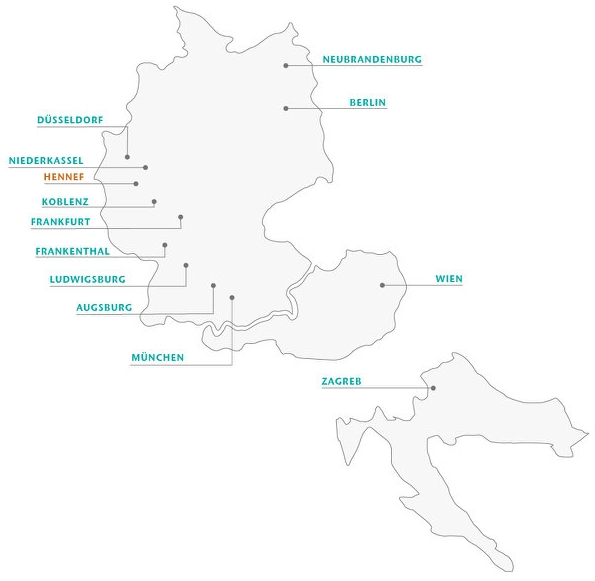
\includegraphics[width = 11cm]{bilder/standorte}
%    \caption{Standorte der CONET Technologies Holding GmbH}
%\end{figure}



%
%\begin{figure}[H]
%  \centering
%    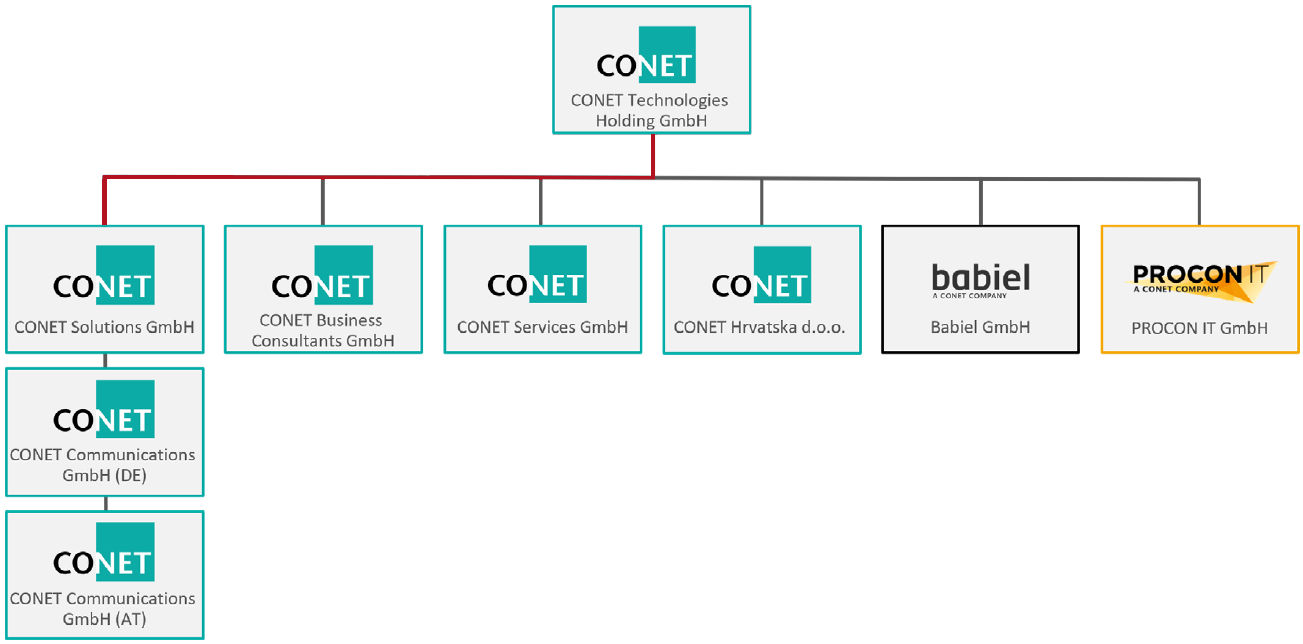
\includegraphics[width = 15cm]{bilder/organigramm_conet}
%    \caption{Unternehmensstruktur CONET Technologies Holding GmbH}
%\end{figure}

%\begin{figure}[H]
%  \centering
%    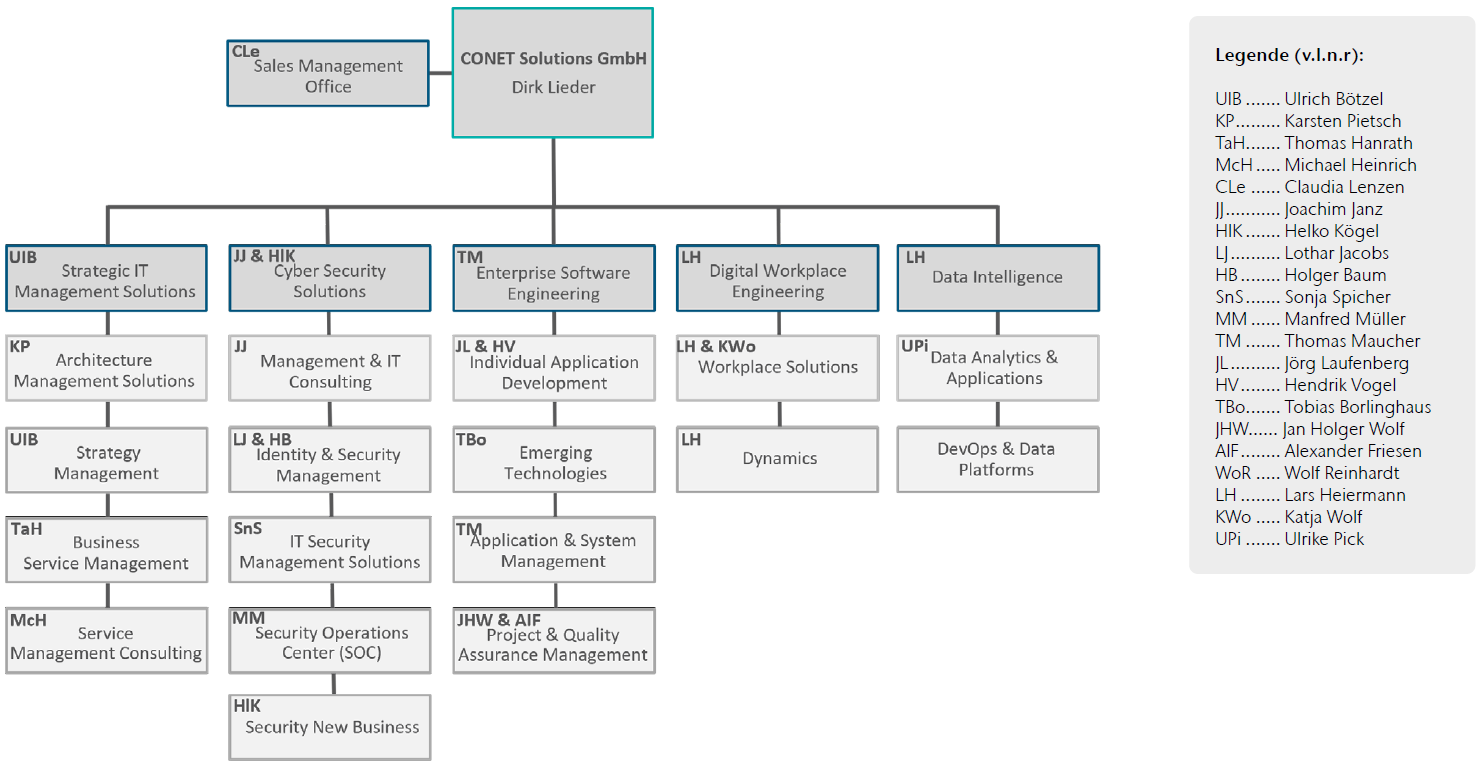
\includegraphics[width = 15cm]{bilder/organigramm_conet_solutions}
%    \caption{Unternehmensstruktur CONET Solutions GmbH}
%\end{figure}

